\documentclass[11pt]{article}

\usepackage[margin=1in]{geometry}
\usepackage[T1]{fontenc}
\usepackage[utf8]{inputenc}
\usepackage{lmodern}
\usepackage{microtype}
\usepackage{amsmath,amssymb,mathtools}
\usepackage{hyperref}
\usepackage{graphicx}
\usepackage{subcaption}
\usepackage{float}
\usepackage{enumitem}
\hypersetup{hidelinks}

\graphicspath{{images/}}

\title{Meeting Notes}
\author{Shreyas Kalvankar}
\date{\today}

\begin{document}
\maketitle

The question is why the evolving NTK helps at smaller widths, but not at larger widths.

\begin{figure}[H]
	\centering
	\begin{subfigure}[t]{0.48\textwidth}
		\centering
		
\includegraphics[width=\linewidth]{train_ls_frozen_vs_evolving_w128.png}
		\caption{Width \(128\).}
	\end{subfigure}
	\hfill
	\begin{subfigure}[t]{0.48\textwidth}
		\centering
		
\includegraphics[width=\linewidth]{train_ls_frozen_vs_evolving_w256.png}
		\caption{Width \(256\).}
	\end{subfigure}

	\vspace{0.6em}

	\begin{subfigure}[t]{0.48\textwidth}
		\centering
		
\includegraphics[width=\linewidth]{train_ls_frozen_vs_evolving_w512.png}
		\caption{Width \(512\).}
	\end{subfigure}
	\hfill
	\begin{subfigure}[t]{0.48\textwidth}
		\centering
		
\includegraphics[width=\linewidth]{train_ls_frozen_vs_evolving_w1024.png}
		\caption{Width \(1024\).}
	\end{subfigure}
	\caption{Least-squares objective comparison across widths. The evolving NTK gives a clear improvement at widths \(128\) and \(256\). The improvement is much smaller at width \(512\), and by width \(1024\) the frozen NTK gives the lower final objective.}
	\label{fig:ls-objective}
\end{figure}

The basic pattern is a width-dependent crossover. At small width, allowing the kernel to evolve improves optimization. At large width, the frozen kernel is already strong enough, and evolving the kernel no longer helps. To understand this, it is natural to first ask whether the evolving dynamics changes the Fourier subspaces themselves.

We therefore start with the projection error
\[
	\|\widehat P_k(t)-P_k\|_F,
\]
which measures how far the learned projector for frequency \(k\) moves away from the reference Fourier projector.

\begin{figure}[H]
	\centering
	\begin{subfigure}[t]{0.78\textwidth}
		\centering
		
\includegraphics[width=\linewidth]{projection_error_absolute_by_freq_w128.png}
		\caption{Width \(128\).}
	\end{subfigure}

	\vspace{0.8em}

	\begin{subfigure}[t]{0.78\textwidth}
		\centering
		
\includegraphics[width=\linewidth]{projection_error_absolute_by_freq_w256.png}
		\caption{Width \(256\).}
	\end{subfigure}
	\caption{Absolute projection error by Fourier subspace for widths \(128\) and \(256\).}
	\label{fig:projection-error-small}
\end{figure}

\begin{figure}[H]
	\centering
	\begin{subfigure}[t]{0.78\textwidth}
		\centering
		
\includegraphics[width=\linewidth]{projection_error_absolute_by_freq_w512.png}
		\caption{Width \(512\).}
	\end{subfigure}

	\vspace{0.8em}

	\begin{subfigure}[t]{0.78\textwidth}
		\centering
		
\includegraphics[width=\linewidth]{projection_error_absolute_by_freq_w1024.png}
		\caption{Width \(1024\).}
	\end{subfigure}
	\caption{Absolute projection error by Fourier subspace for widths \(512\) and \(1024\).}
	\label{fig:projection-error-large}
\end{figure}


\begin{figure}[H]
	\centering
	\begin{subfigure}[t]{0.78\textwidth}
		\centering
		
\includegraphics[width=\linewidth]{rms_cos_alignment_by_freq_w128.png}
		\caption{Width \(128\).}
	\end{subfigure}

	\vspace{0.8em}

	\begin{subfigure}[t]{0.78\textwidth}
		\centering
		
\includegraphics[width=\linewidth]{rms_cos_alignment_by_freq_w256.png}
		\caption{Width \(256\).}
	\end{subfigure}
	\caption{RMS-cos alignment by Fourier subspace for widths \(128\) and \(256\).}
	\label{fig:alignment-small}
\end{figure}

\begin{figure}[H]
	\centering
	\begin{subfigure}[t]{0.78\textwidth}
		\centering
		
\includegraphics[width=\linewidth]{rms_cos_alignment_by_freq_w512.png}
		\caption{Width \(512\).}
	\end{subfigure}

	\vspace{0.8em}

	\begin{subfigure}[t]{0.78\textwidth}
		\centering
		
\includegraphics[width=\linewidth]{rms_cos_alignment_by_freq_w1024.png}
		\caption{Width \(1024\).}
	\end{subfigure}
	\caption{RMS-cos alignment by Fourier subspace for widths \(512\) and \(1024\).}
	\label{fig:alignment-large}
\end{figure}

The projection-error and cosine alignment plots show a consistent geometric trend.
Under the evolving dynamics, several higher-frequency subspaces move away
from their Fourier reference subspaces. The projection-error plots show this as
an increase in \(\|\widehat P_k(t)-P_k\|_F\), while the cos alignment plots
show it as a drop in subspace alignment.

This rules out a simple explanation based on improved Fourier geometry. The
evolving NTK does not help because it becomes more Fourier-aligned. If anything,
it becomes less Fourier-aligned, especially for higher frequencies. The main
difference across widths is the starting point. At low width, the frozen NTK
already starts with worse Fourier geometry; at high width, it starts much closer
to the Fourier reference. Thus, at high width, feature learning moves the kernel
away from a better initial geometry.

Therefore, projection error and cosine alignment should be read mainly as
geometry diagnostics. They show that feature learning changes the Fourier
subspaces, but they do not by themselves explain why the evolving model reaches
lower loss at small width. To understand the loss, we also need to know how
strongly the kernel acts in the directions being fitted. This is the distinction
between geometry and strength.

A small toy example makes this point clearer. Let
\[
	\mathcal F_1=\operatorname{span}\{e_1,e_2\}
\]
be a Fourier subspace, and let \(e_3\) represent another frequency. Rotating the
basis inside \(\mathcal F_1\) does not change the subspace, and therefore does
not change the projector \(P_1\). Projection error appears only when the subspace
itself tilts into another frequency direction. For example, suppose the learned
subspace is
\[
	\widehat{\mathcal F}_1
	=
	\operatorname{span}\{\cos\theta\,e_1+\sin\theta\,e_3,\ e_2\}.
\]
Then \(\widehat{\mathcal F}_1\neq \mathcal F_1\), and
\[
	\|\widehat P_1-P_1\|_F
	=
	\sqrt{2}\sin\theta .
\]
So this is genuinely worse Fourier alignment: the learned frequency block is no
longer purely the original Fourier block.

However, worse alignment does not automatically mean slower loss decay. To see
this, consider the two-dimensional slice \(\operatorname{span}\{e_1,e_3\}\),
where \(e_1\) is a Fourier direction and \(e_3\) represents a direction outside
the original Fourier subspace. Suppose the residual is mainly in the Fourier
direction
\[
	r=e_1
	=
	\begin{pmatrix}
		1 \\
		0
	\end{pmatrix}.
\]
A frozen, Fourier-aligned kernel may act on this slice as
\[
	K_{\mathrm{frozen}}
	=
	\begin{pmatrix}
		1 & 0   \\
		0 & 0.1
	\end{pmatrix}.
\]
Then
\[
	\langle e_1,K_{\mathrm{frozen}}e_1\rangle
	=
	1.
\]

Now suppose the evolving kernel tilts the leading eigendirection away from
\(e_1\) and toward \(e_3\). Let
\[
	R_\theta
	=
	\begin{pmatrix}
		\cos\theta & -\sin\theta \\
		\sin\theta & \cos\theta
	\end{pmatrix}.
\]
The first tilted eigenvector is
\[
	u_1=\cos\theta\,e_1+\sin\theta\,e_3.
\]
This is not a rotation inside the same Fourier subspace. It is a tilt into
another frequency direction, so it would increase projection error.

Assume that the evolving kernel is diagonal in this tilted eigenbasis, with a
larger leading eigenvalue:
\[
	K_{\mathrm{evolving}}
	=
	R_\theta
	\begin{pmatrix}
		3 & 0   \\
		0 & 0.1
	\end{pmatrix}
	R_\theta^\top .
\]
In the original \((e_1,e_3)\) basis, this is
\[
	K_{\mathrm{evolving}}
	=
	\begin{pmatrix}
		3\cos^2\theta+0.1\sin^2\theta
		 &
		(3-0.1)\sin\theta\cos\theta
		\\
		(3-0.1)\sin\theta\cos\theta
		 &
		3\sin^2\theta+0.1\cos^2\theta
	\end{pmatrix}.
\]
So for the same residual \(r=e_1\),
\[
	\langle e_1,K_{\mathrm{evolving}}e_1\rangle
	=
	3\cos^2\theta+0.1\sin^2\theta .
\]
For \(\theta=30^\circ\), this gives
\[
	3\cdot 0.75+0.1\cdot 0.25
	=
	2.275,
\]
which is larger than the frozen value \(1\). Thus the evolving kernel can be
less Fourier-aligned and still remove this residual direction faster, because
the larger eigenvalue more than compensates for the tilt.

The example is not meant to prove that this is exactly what happens in the
experiment. It only explains why the geometry plots are incomplete. Projection
error and RMS-cos alignment measure whether the Fourier subspaces move. They do
not measure whether the kernel becomes stronger along the directions that still
matter for the residual. This motivates the next diagnostic: spectral strength.

For each Fourier block \(\mathcal F_k\), we summarize the average kernel strength by
\[
	\mu_{\mathcal F_k}(t)
	=
	\frac{1}{d_k}
	\operatorname{tr}\!\left(P_k K_t P_k\right),
\]
where \(P_k\) is the projector onto the \(k\)-th Fourier subspace and \(d_k=\dim(\mathcal F_k)\). This is not an individual eigenvalue; it is the average spectral strength inside the subspace.

\begin{figure}[H]
	\centering
	\begin{subfigure}[t]{0.78\textwidth}
		\centering
		
\includegraphics[width=\linewidth]{spectral_strength_by_freq_w128.png}
		\caption{Width \(128\).}
	\end{subfigure}

	\vspace{0.8em}

	\begin{subfigure}[t]{0.78\textwidth}
		\centering
		
\includegraphics[width=\linewidth]{spectral_strength_by_freq_w256.png}
		\caption{Width \(256\).}
	\end{subfigure}
	\caption{Per-frequency spectral strength for widths \(128\) and \(256\).}
	\label{fig:spectral-strength-small}
\end{figure}

\begin{figure}[H]
	\centering
	\begin{subfigure}[t]{0.78\textwidth}
		\centering
		
\includegraphics[width=\linewidth]{spectral_strength_by_freq_w512.png}
		\caption{Width \(512\).}
	\end{subfigure}

	\vspace{0.8em}

	\begin{subfigure}[t]{0.78\textwidth}
		\centering
		
\includegraphics[width=\linewidth]{spectral_strength_by_freq_w1024.png}
		\caption{Width \(1024\).}
	\end{subfigure}
	\caption{Per-frequency spectral strength for widths \(512\) and \(1024\).}
	\label{fig:spectral-strength-large}
\end{figure}

The spectral-strength plots give the missing part of the story. Across the
different target-amplitude settings, the evolving NTK consistently increases the
average kernel strength in the low-frequency blocks, especially \(k=0\) and
\(k=1\), with a smaller increase for \(k=2\). The higher-frequency blocks remain
much weaker. This is important because the same qualitative pattern appears even
when the target amplitudes are changed: the low-frequency boost is not simply an
artifact of assigning the largest amplitude to the constant or lowest-frequency
mode.

This suggests that the evolving kernel has a robust tendency to reweight spectral
strength toward low frequencies. The geometry plots showed the cost: feature
learning moves the Fourier subspaces and worsens alignment, especially for higher
frequencies. The spectral-strength plots show the possible benefit: the same
evolution also increases kernel strength in the low-frequency blocks. Thus the
evolving NTK can improve the loss at small width despite worse Fourier geometry.

The width dependence is then naturally interpreted as a tradeoff. At low width,
the frozen NTK is a rougher finite-width approximation, so the extra
low-frequency strength gained through feature learning can outweigh the geometric
drift. At high width, the frozen NTK starts closer to the Fourier reference and
is already a strong baseline. The additional spectral reweighting from feature
learning is then less useful relative to the cost of moving away from the
Fourier geometry. This gives a plausible explanation for the crossover: feature
learning helps when the low-frequency spectral gain is large enough to compensate
for subspace drift, but loses its advantage once the frozen kernel is already
stable and sufficiently strong.

A concise takeaway is:
\begin{quote}
	Feature learning does not help by preserving the Fourier geometry. The
	projection-error and cosine-alignment plots show the opposite: the evolving
	kernel moves the Fourier subspaces, especially at higher frequencies. The
	benefit appears to come from spectral reweighting instead. Across the
	amplitude variants, the evolving NTK increases low-frequency kernel strength,
	especially for \(k=0\) and \(k=1\). At small width, this gain can outweigh
	the geometric drift. At large width, the frozen NTK is already a good and
	stable approximation, so the extra gain from feature learning is no longer
	enough to compensate for the drift.
\end{quote}

\begin{figure}[H]
	\centering
	\begin{subfigure}[t]{0.82\textwidth}
		\centering
		
\includegraphics[width=\linewidth]{spectral_strength_by_freq_w128.png}
		\caption{Original amplitudes.}
	\end{subfigure}

	\vspace{0.8em}

	\begin{subfigure}[t]{0.82\textwidth}
		\centering
		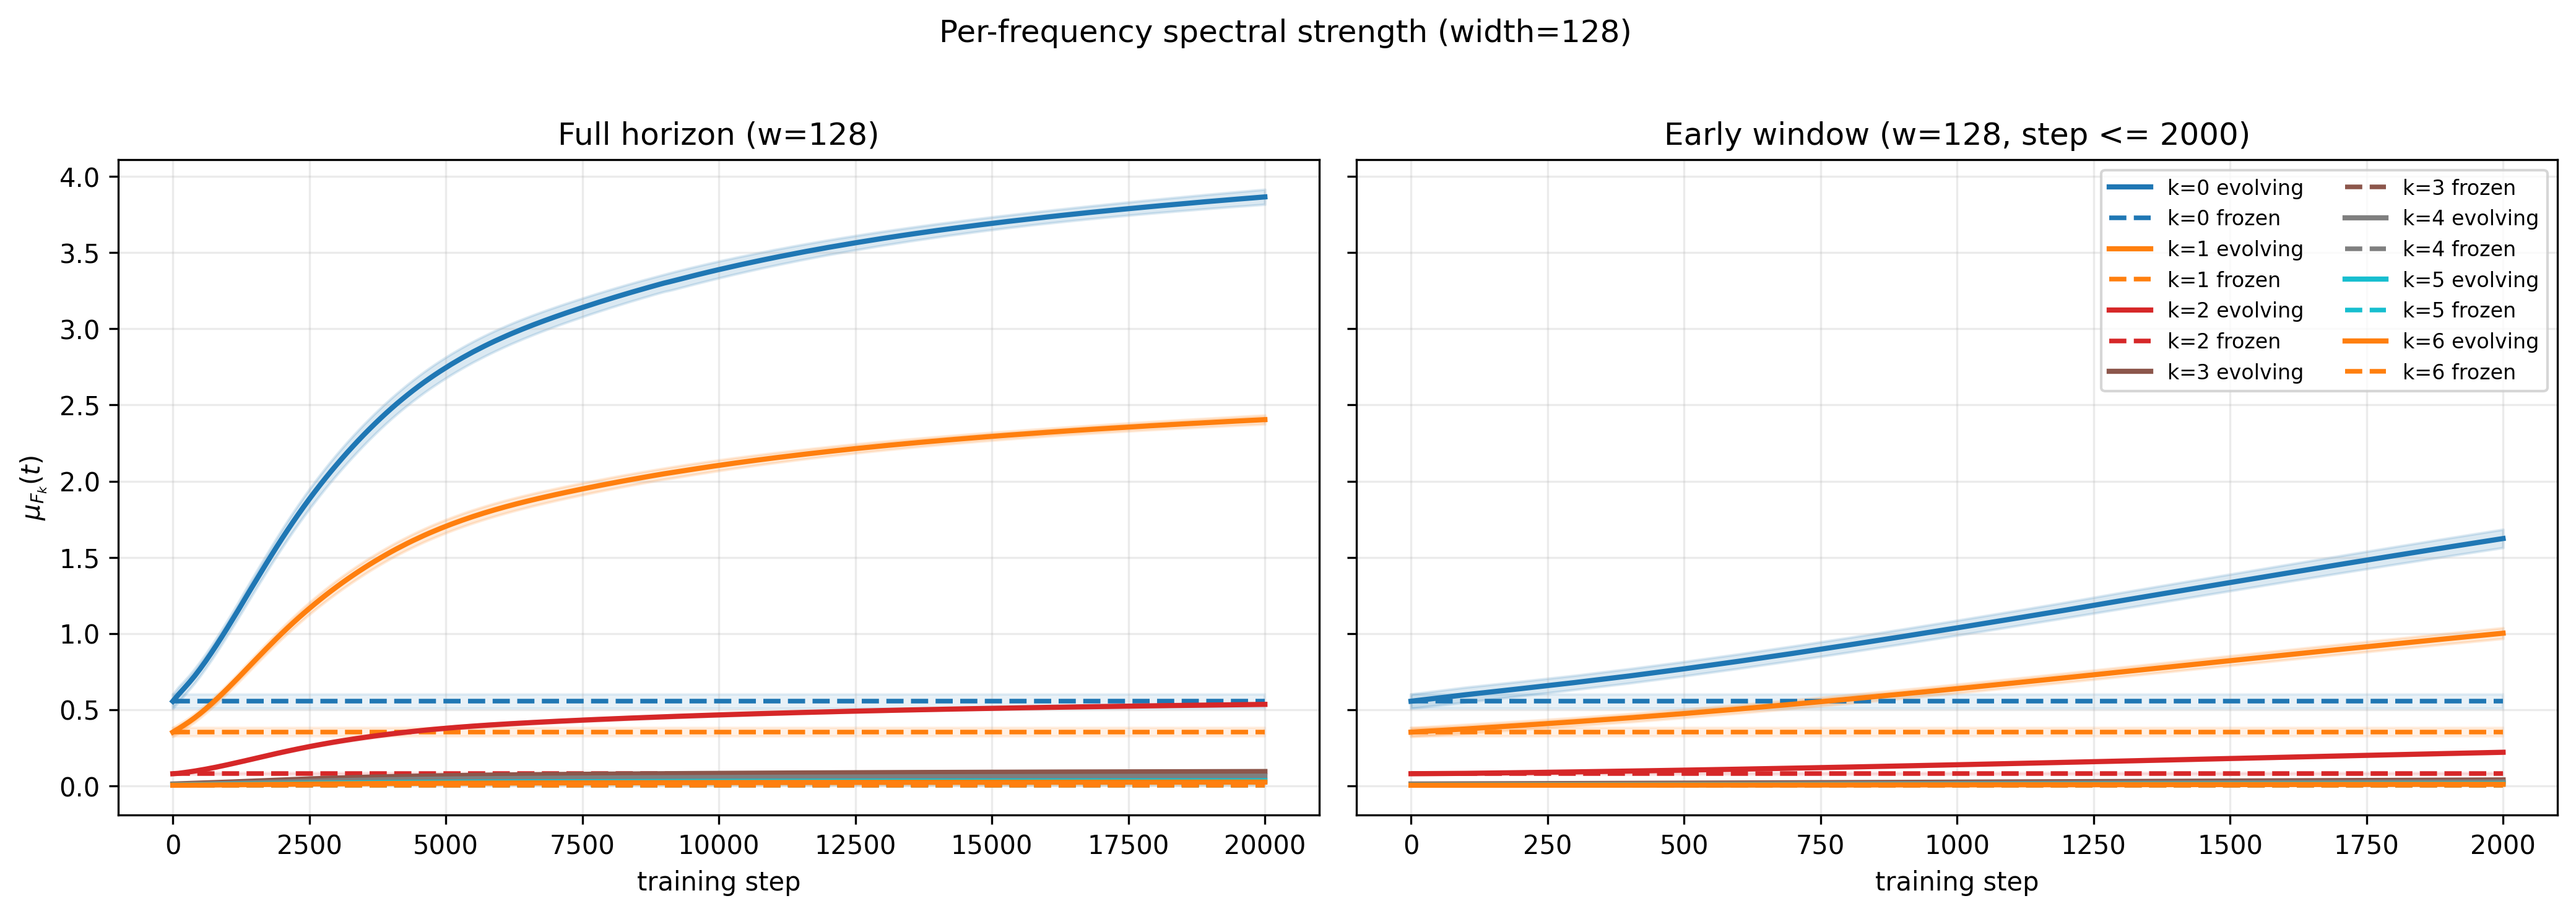
\includegraphics[width=\linewidth]{spectral_strength_equalamp_by_freq_w128.png}
		\caption{Equal amplitudes.}
	\end{subfigure}

	\vspace{0.8em}

	\begin{subfigure}[t]{0.82\textwidth}
		\centering
		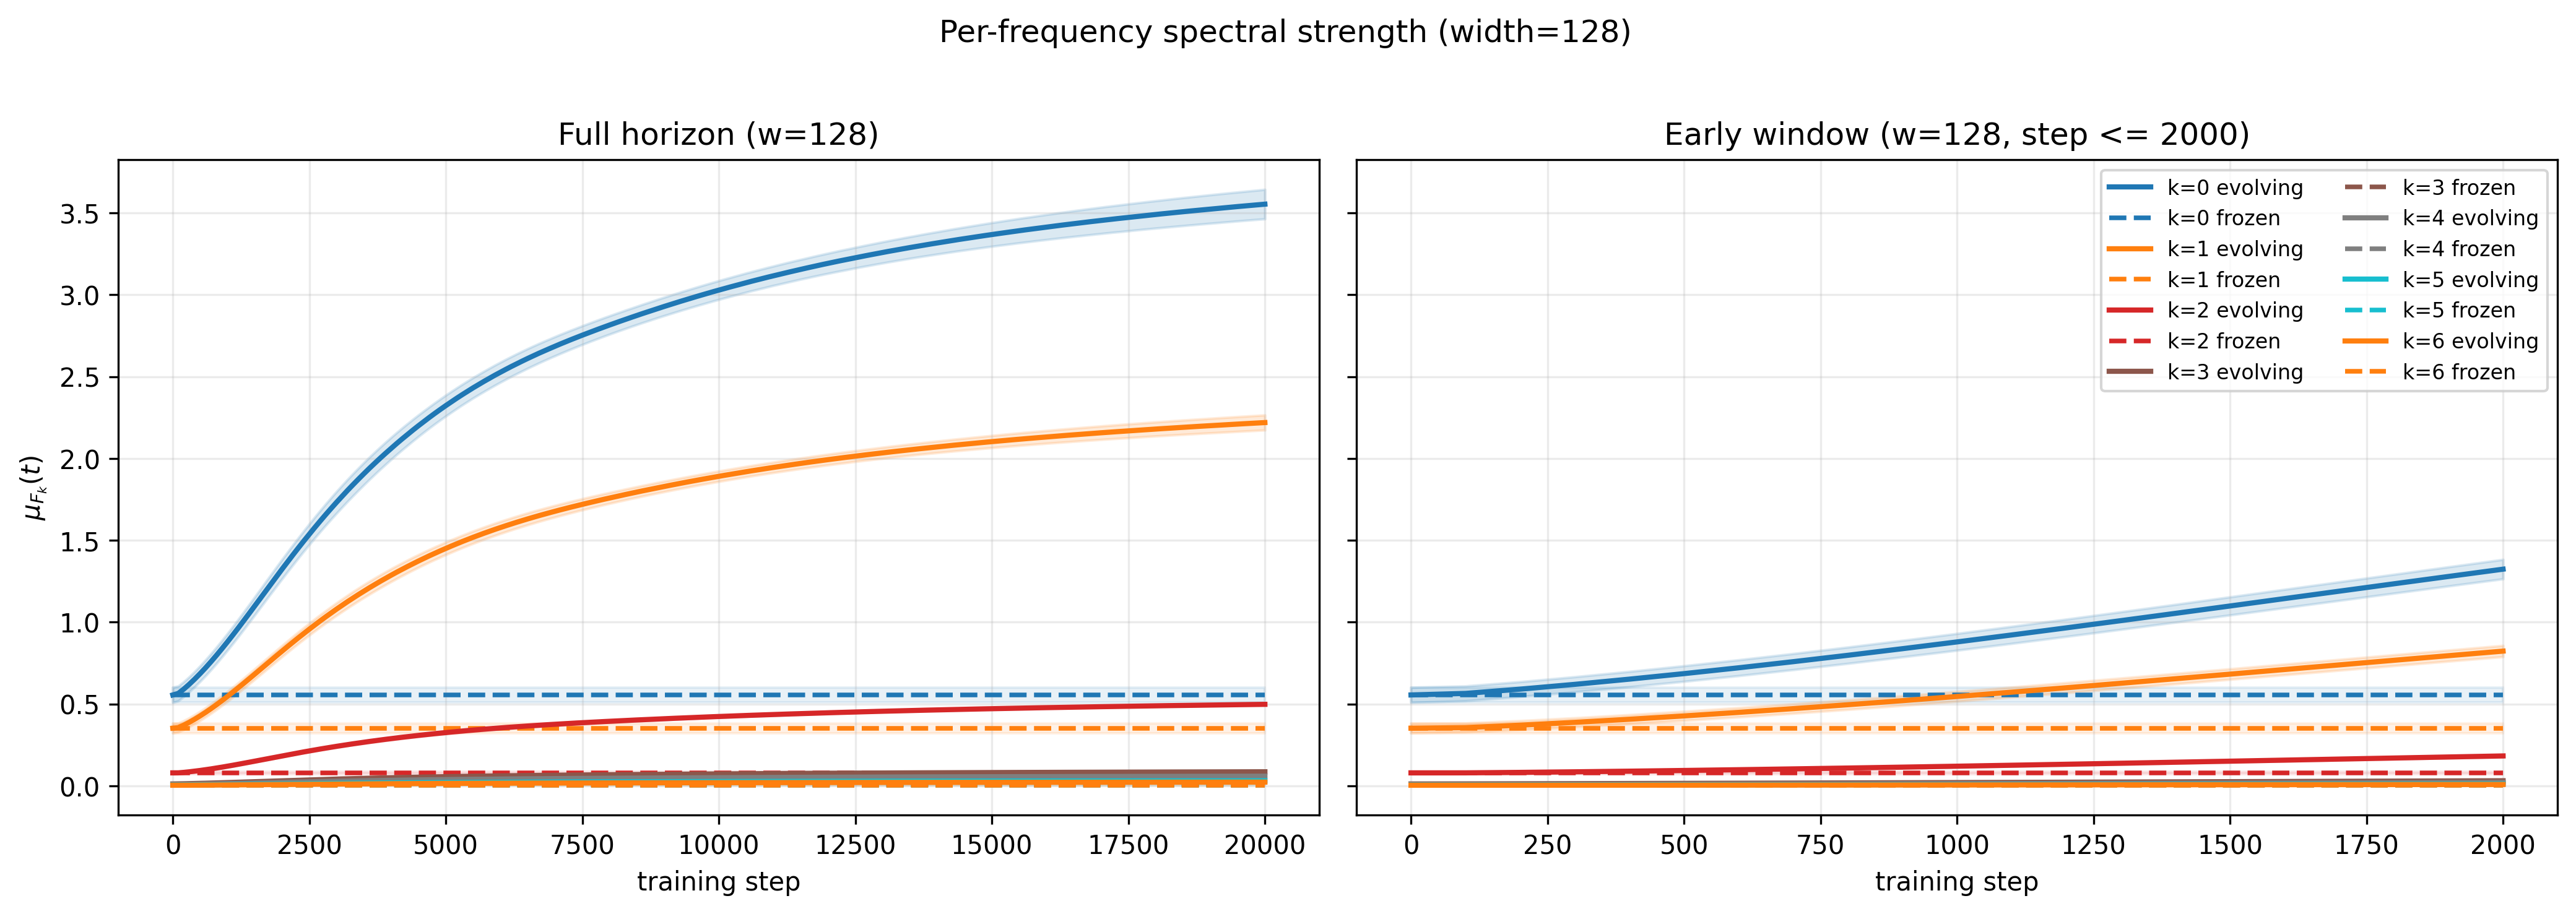
\includegraphics[width=\linewidth]{spectral_strength_revamp_by_freq_w128.png}
		\caption{Reversed amplitudes.}
	\end{subfigure}
	\caption{Per-frequency spectral strength at width \(128\) under the three target-amplitude settings.}
	\label{fig:spectral-strength-w128-all}
\end{figure}

\begin{figure}[H]
	\centering
	\begin{subfigure}[t]{0.82\textwidth}
		\centering
		
\includegraphics[width=\linewidth]{spectral_strength_by_freq_w256.png}
		\caption{Original amplitudes.}
	\end{subfigure}

	\vspace{0.8em}

	\begin{subfigure}[t]{0.82\textwidth}
		\centering
		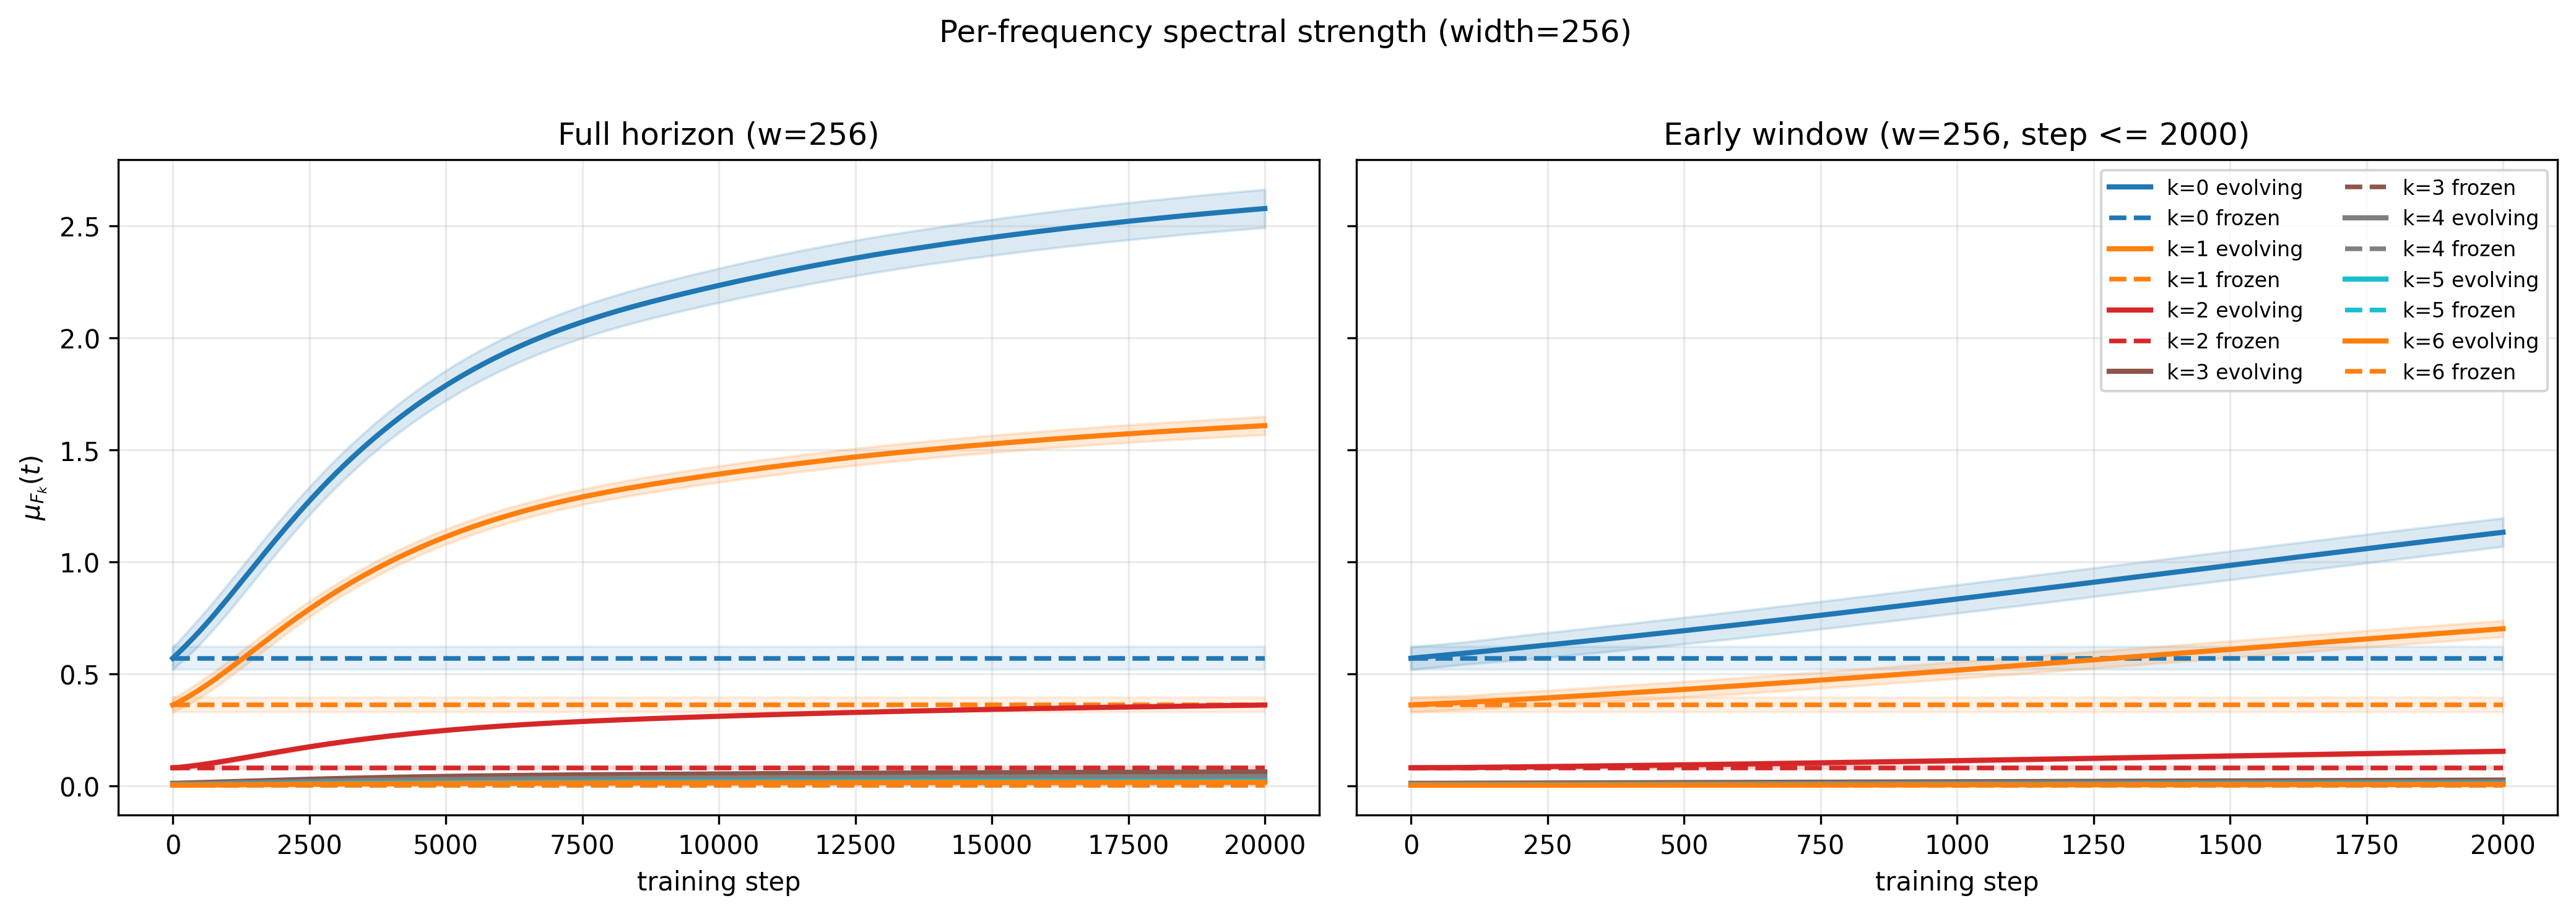
\includegraphics[width=\linewidth]{spectral_strength_equalamp_by_freq_w256.png}
		\caption{Equal amplitudes.}
	\end{subfigure}

	\vspace{0.8em}

	\begin{subfigure}[t]{0.82\textwidth}
		\centering
		
\includegraphics[width=\linewidth]{spectral_strength_revamp_by_freq_w256.png}
		\caption{Reversed amplitudes.}
	\end{subfigure}
	\caption{Per-frequency spectral strength at width \(256\) under the three target-amplitude settings.}
	\label{fig:spectral-strength-w256-all}
\end{figure}

\begin{figure}[H]
	\centering
	\begin{subfigure}[t]{0.82\textwidth}
		\centering
		
\includegraphics[width=\linewidth]{spectral_strength_by_freq_w512.png}
		\caption{Original amplitudes.}
	\end{subfigure}

	\vspace{0.8em}

	\begin{subfigure}[t]{0.82\textwidth}
		\centering
		
\includegraphics[width=\linewidth]{spectral_strength_equalamp_by_freq_w512.png}
		\caption{Equal amplitudes.}
	\end{subfigure}

	\vspace{0.8em}

	\begin{subfigure}[t]{0.82\textwidth}
		\centering
		
\includegraphics[width=\linewidth]{spectral_strength_revamp_by_freq_w512.png}
		\caption{Reversed amplitudes.}
	\end{subfigure}
	\caption{Per-frequency spectral strength at width \(512\) under the three target-amplitude settings.}
	\label{fig:spectral-strength-w512-all}
\end{figure}

\begin{figure}[H]
	\centering
	\begin{subfigure}[t]{0.82\textwidth}
		\centering
		
\includegraphics[width=\linewidth]{spectral_strength_by_freq_w1024.png}
		\caption{Original amplitudes.}
	\end{subfigure}

	\vspace{0.8em}

	\begin{subfigure}[t]{0.82\textwidth}
		\centering
		
\includegraphics[width=\linewidth]{spectral_strength_equalamp_by_freq_w1024.png}
		\caption{Equal amplitudes.}
	\end{subfigure}

	\vspace{0.8em}

	\begin{subfigure}[t]{0.82\textwidth}
		\centering
		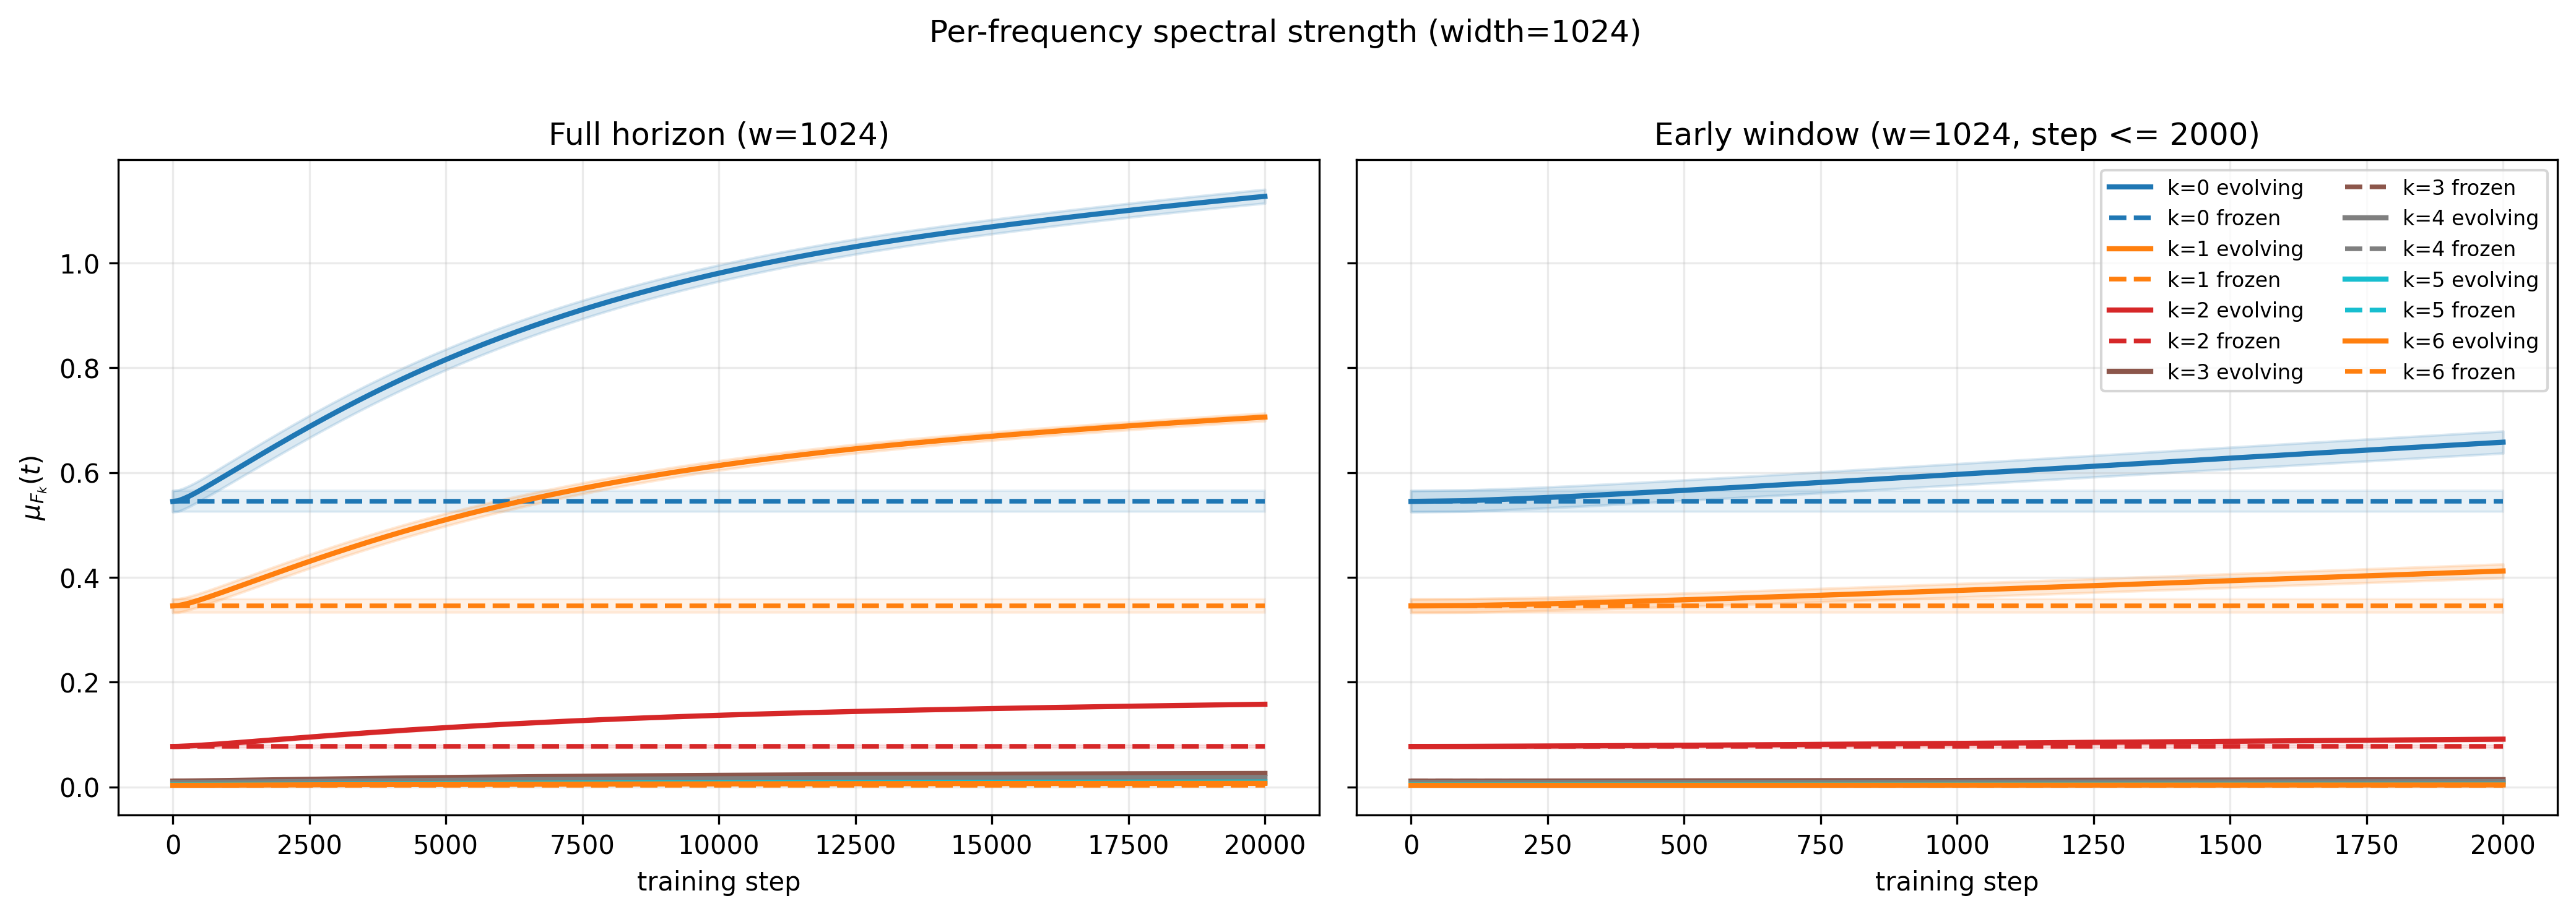
\includegraphics[width=\linewidth]{spectral_strength_revamp_by_freq_w1024.png}
		\caption{Reversed amplitudes.}
	\end{subfigure}
	\caption{Per-frequency spectral strength at width \(1024\) under the three target-amplitude settings.}
	\label{fig:spectral-strength-w1024-all}
\end{figure}

\begin{figure}[H]
	\centering
	\begin{subfigure}[t]{0.48\textwidth}
		\centering
		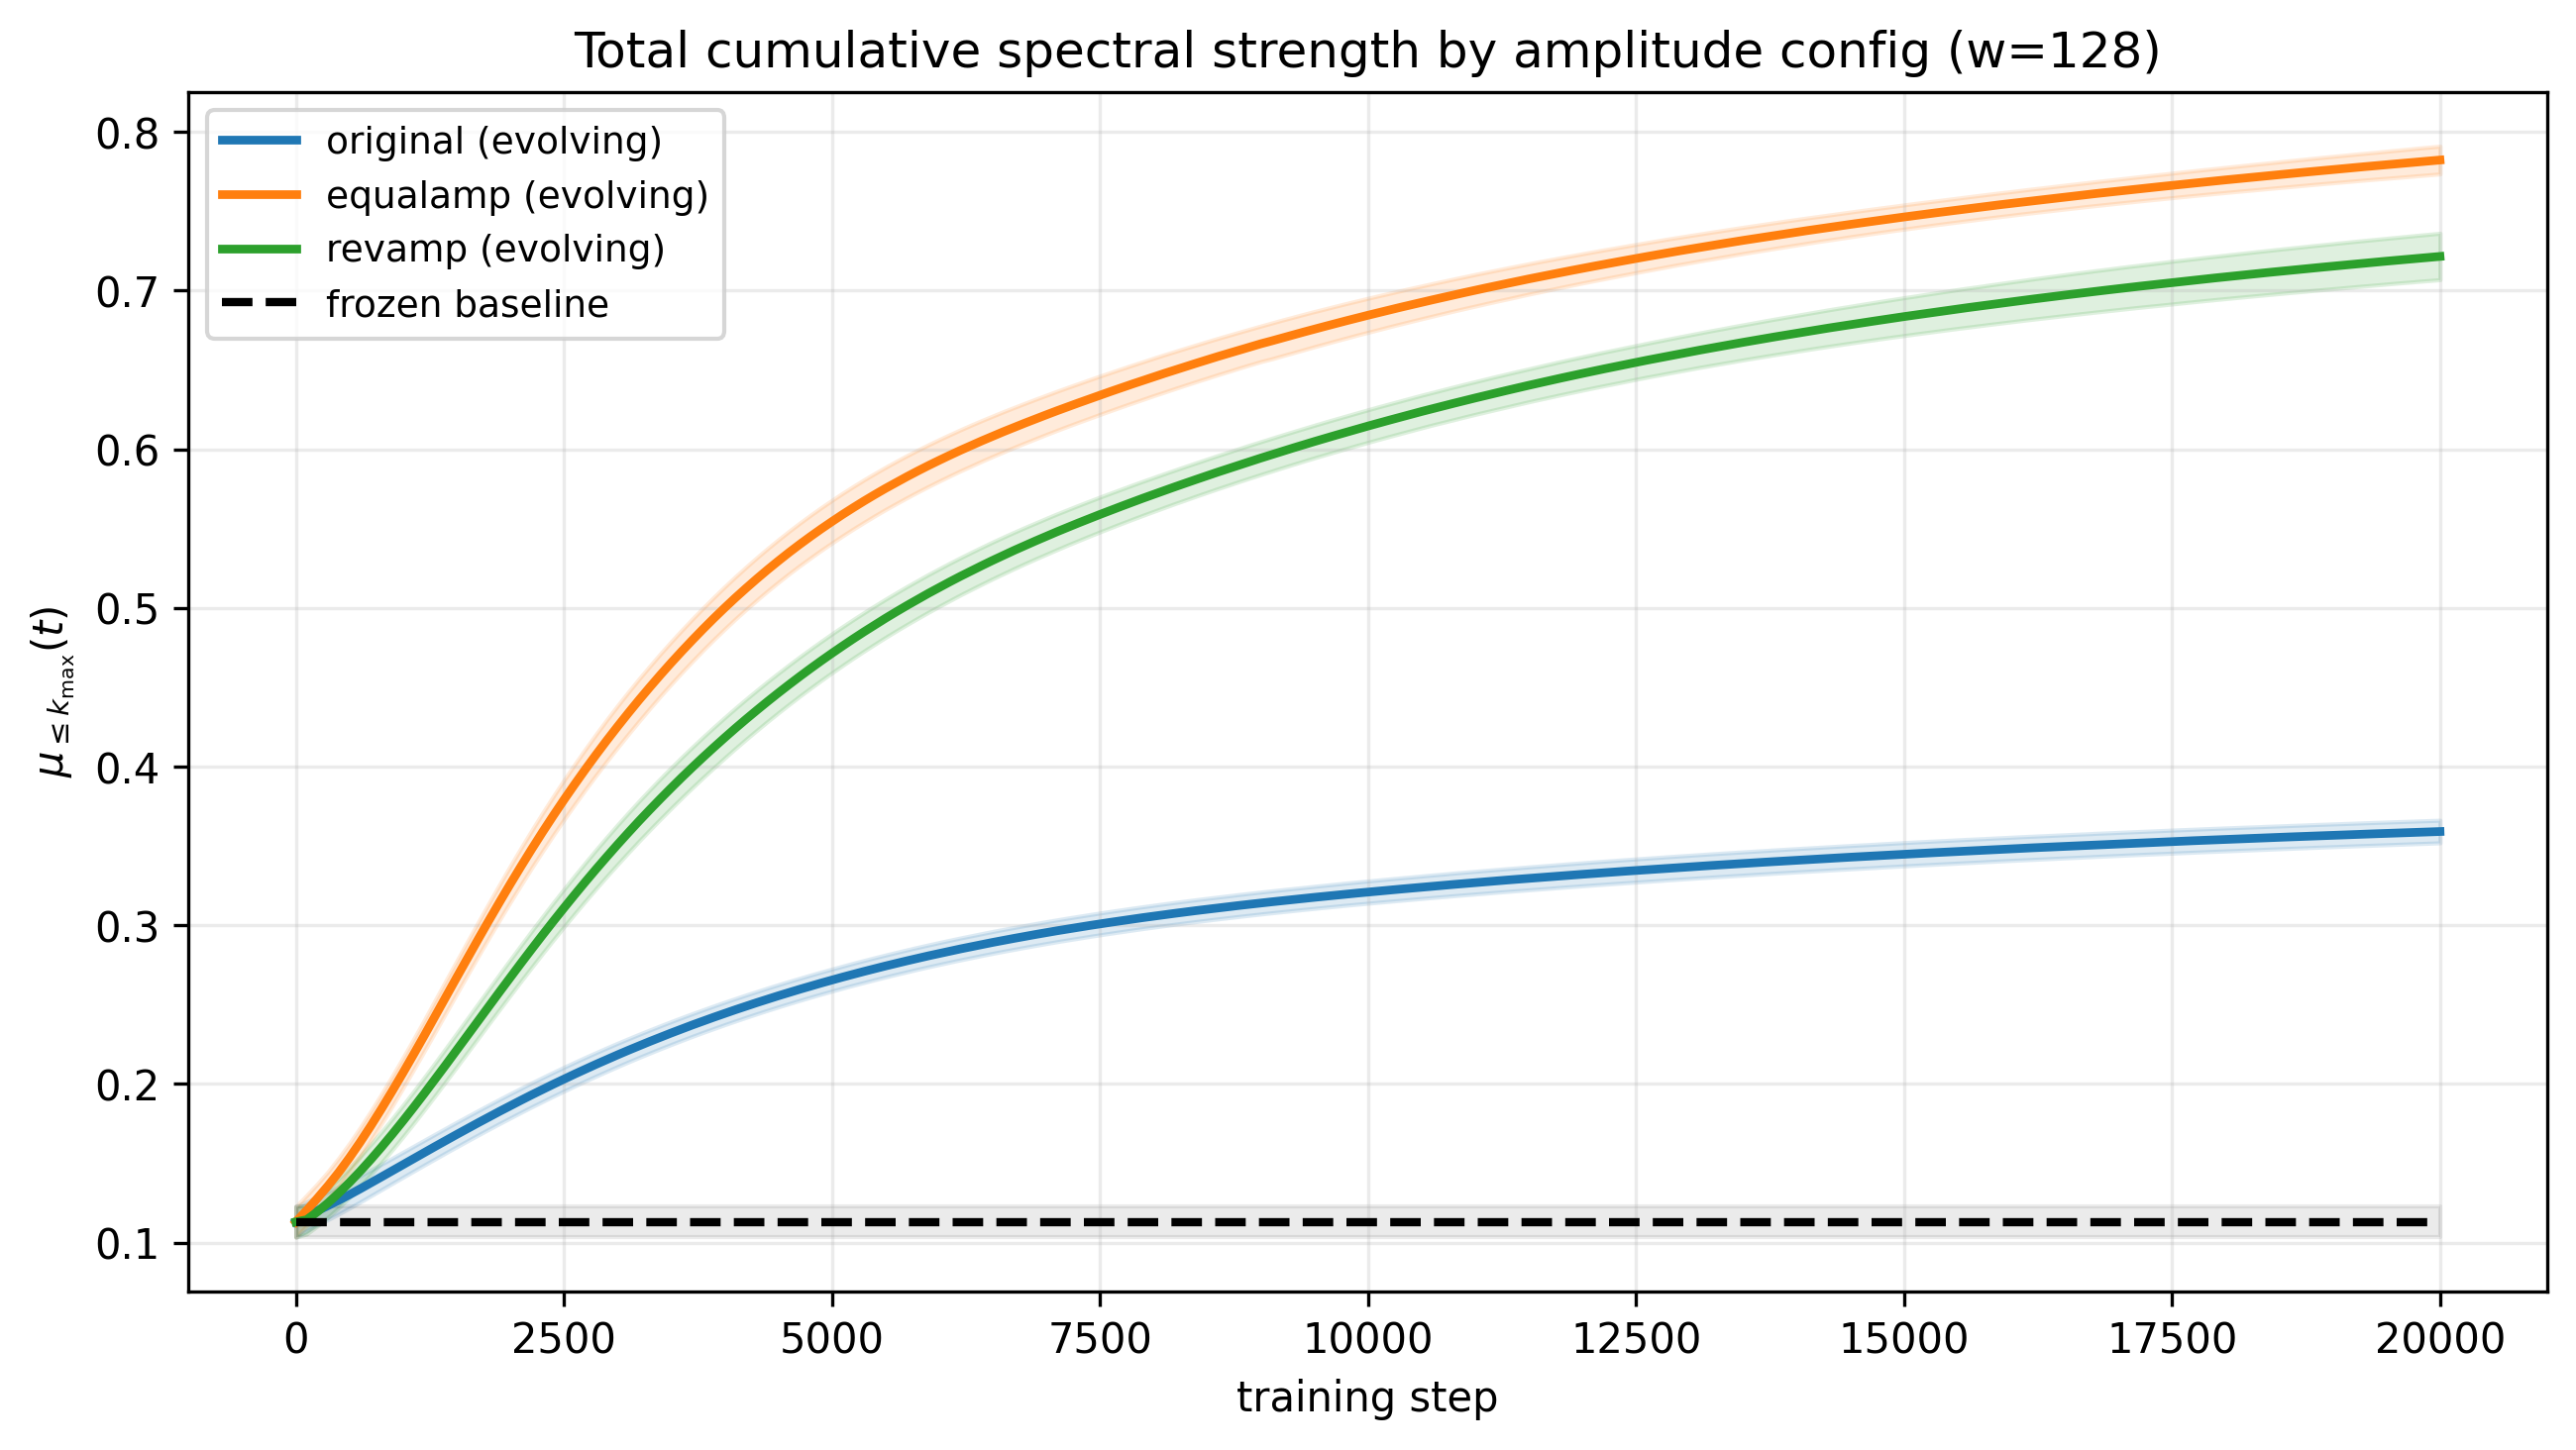
\includegraphics[width=\linewidth]{total_cumulative_mu_amp_configs_w128.png}
		\caption{Width \(128\).}
	\end{subfigure}
	\hfill
	\begin{subfigure}[t]{0.48\textwidth}
		\centering
		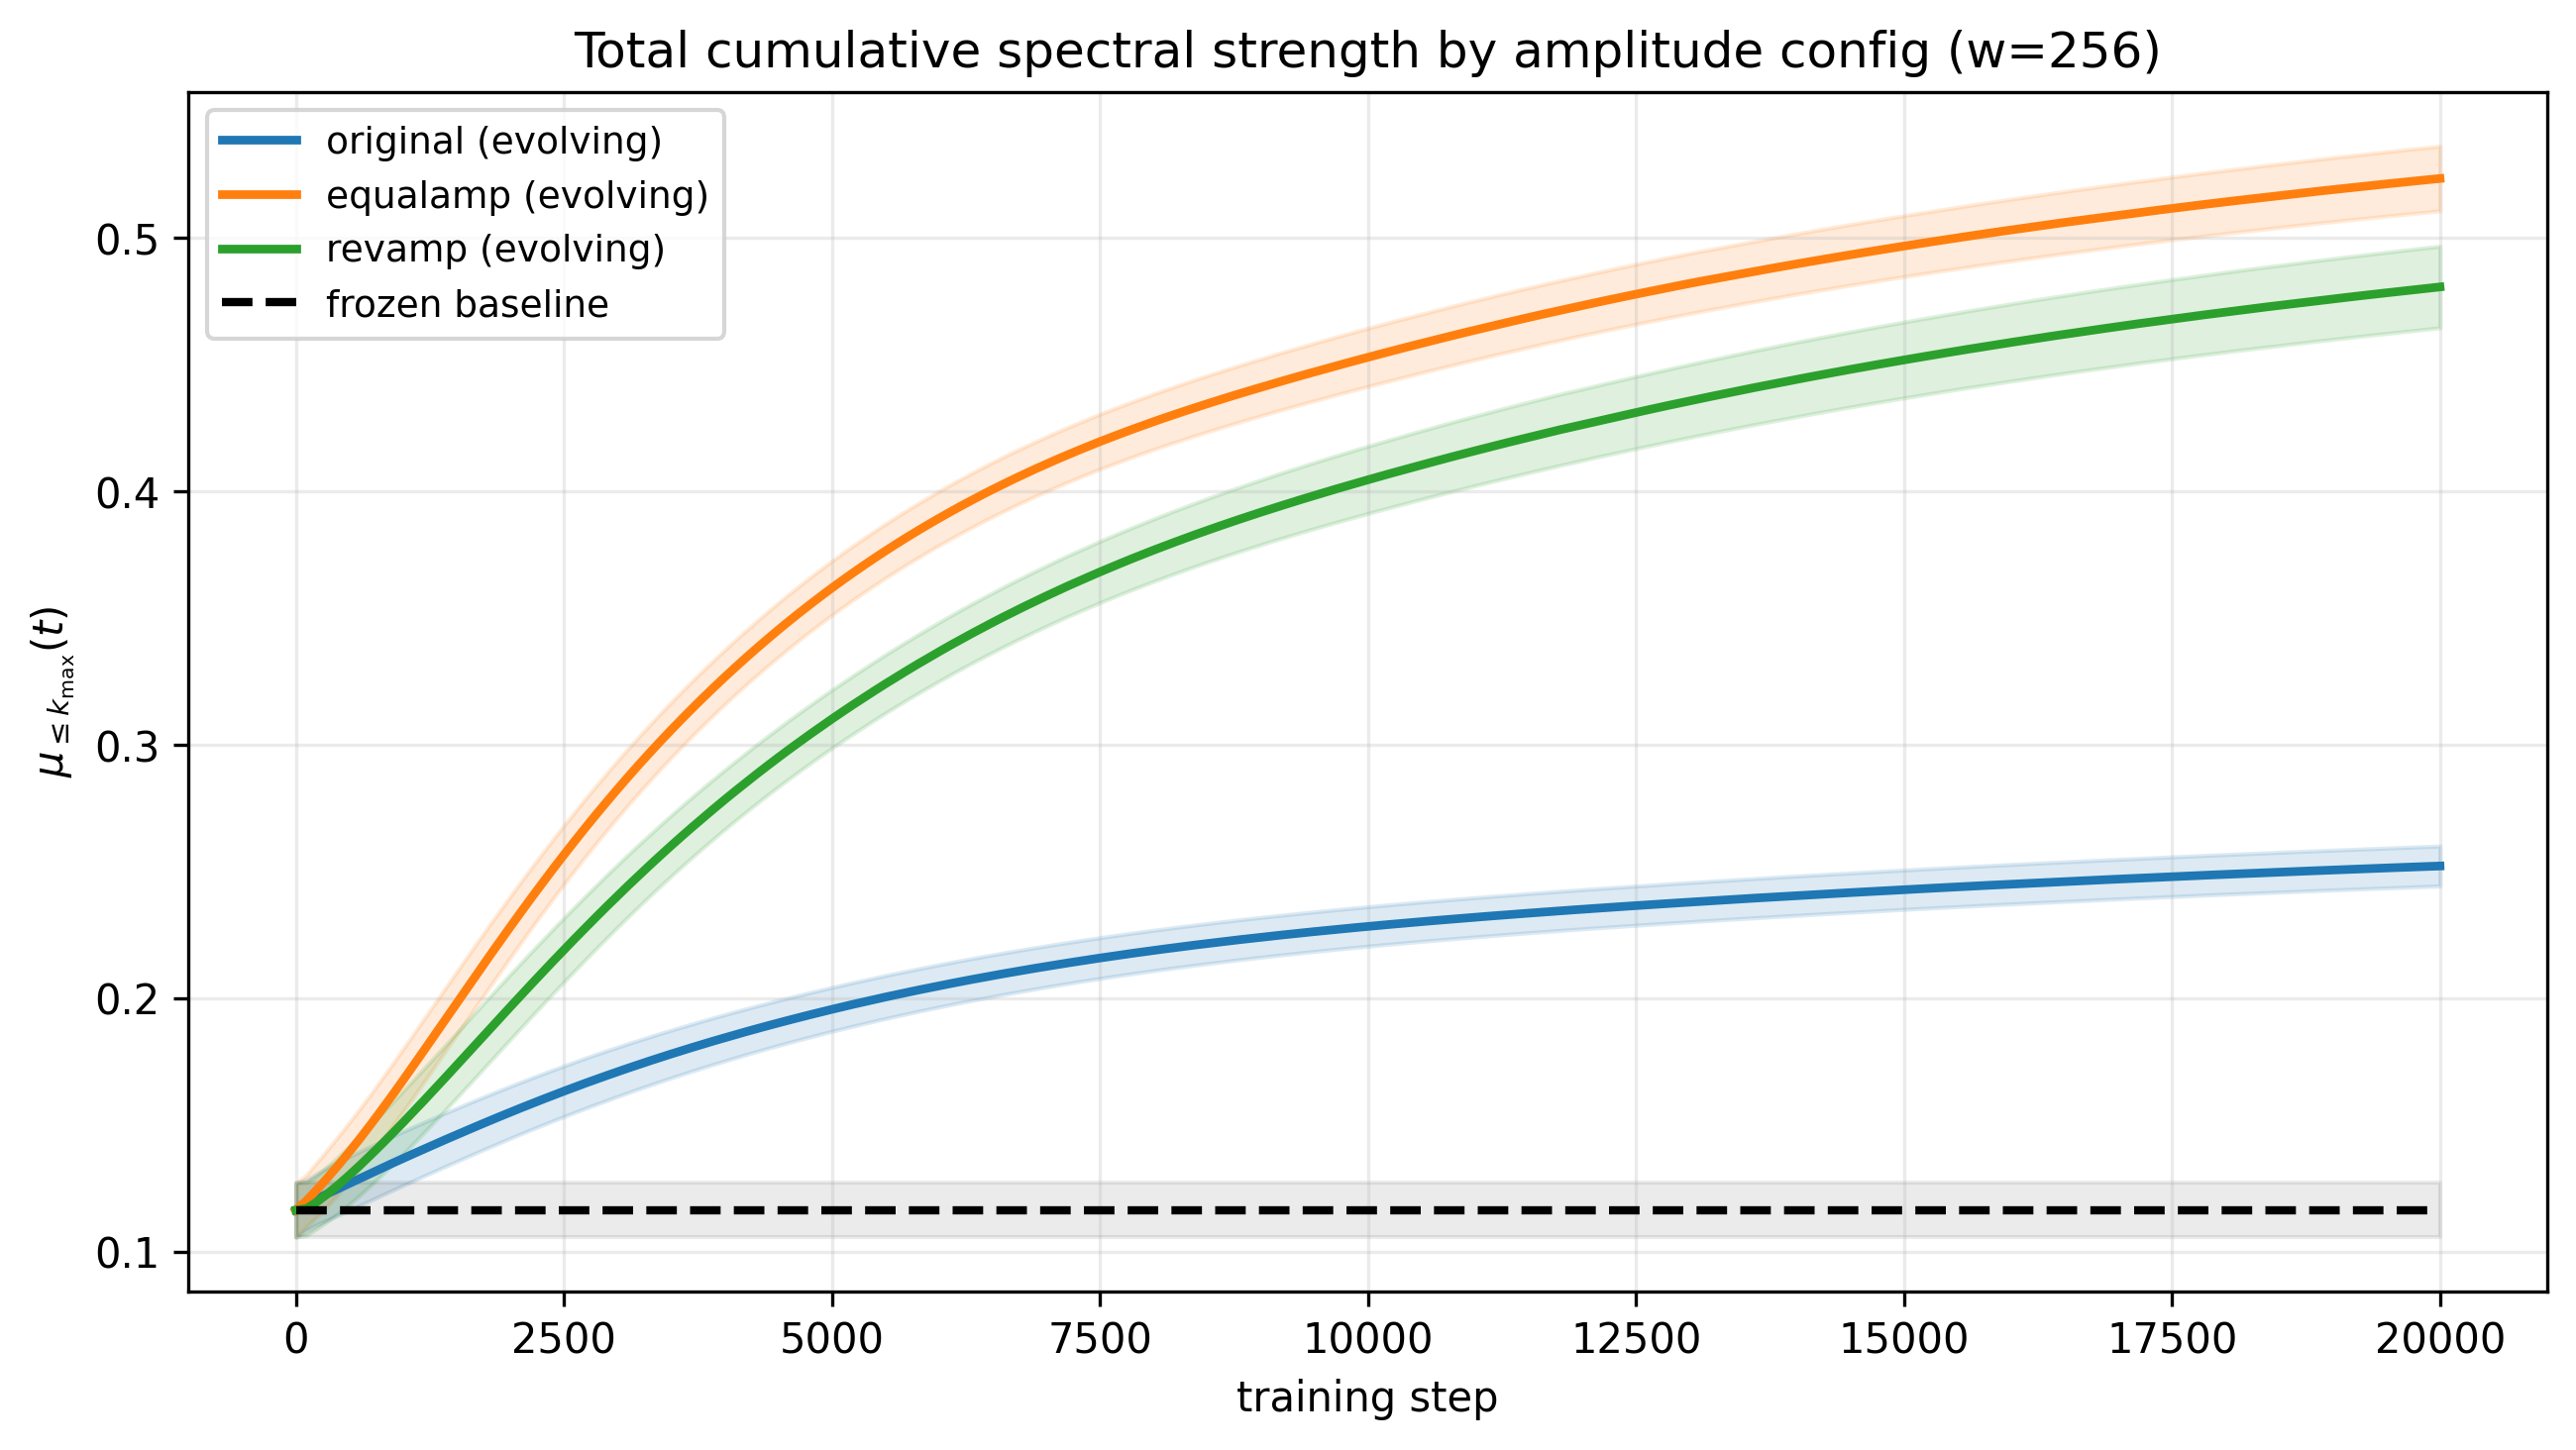
\includegraphics[width=\linewidth]{total_cumulative_mu_amp_configs_w256.png}
		\caption{Width \(256\).}
	\end{subfigure}

	\vspace{0.8em}

	\begin{subfigure}[t]{0.48\textwidth}
		\centering
		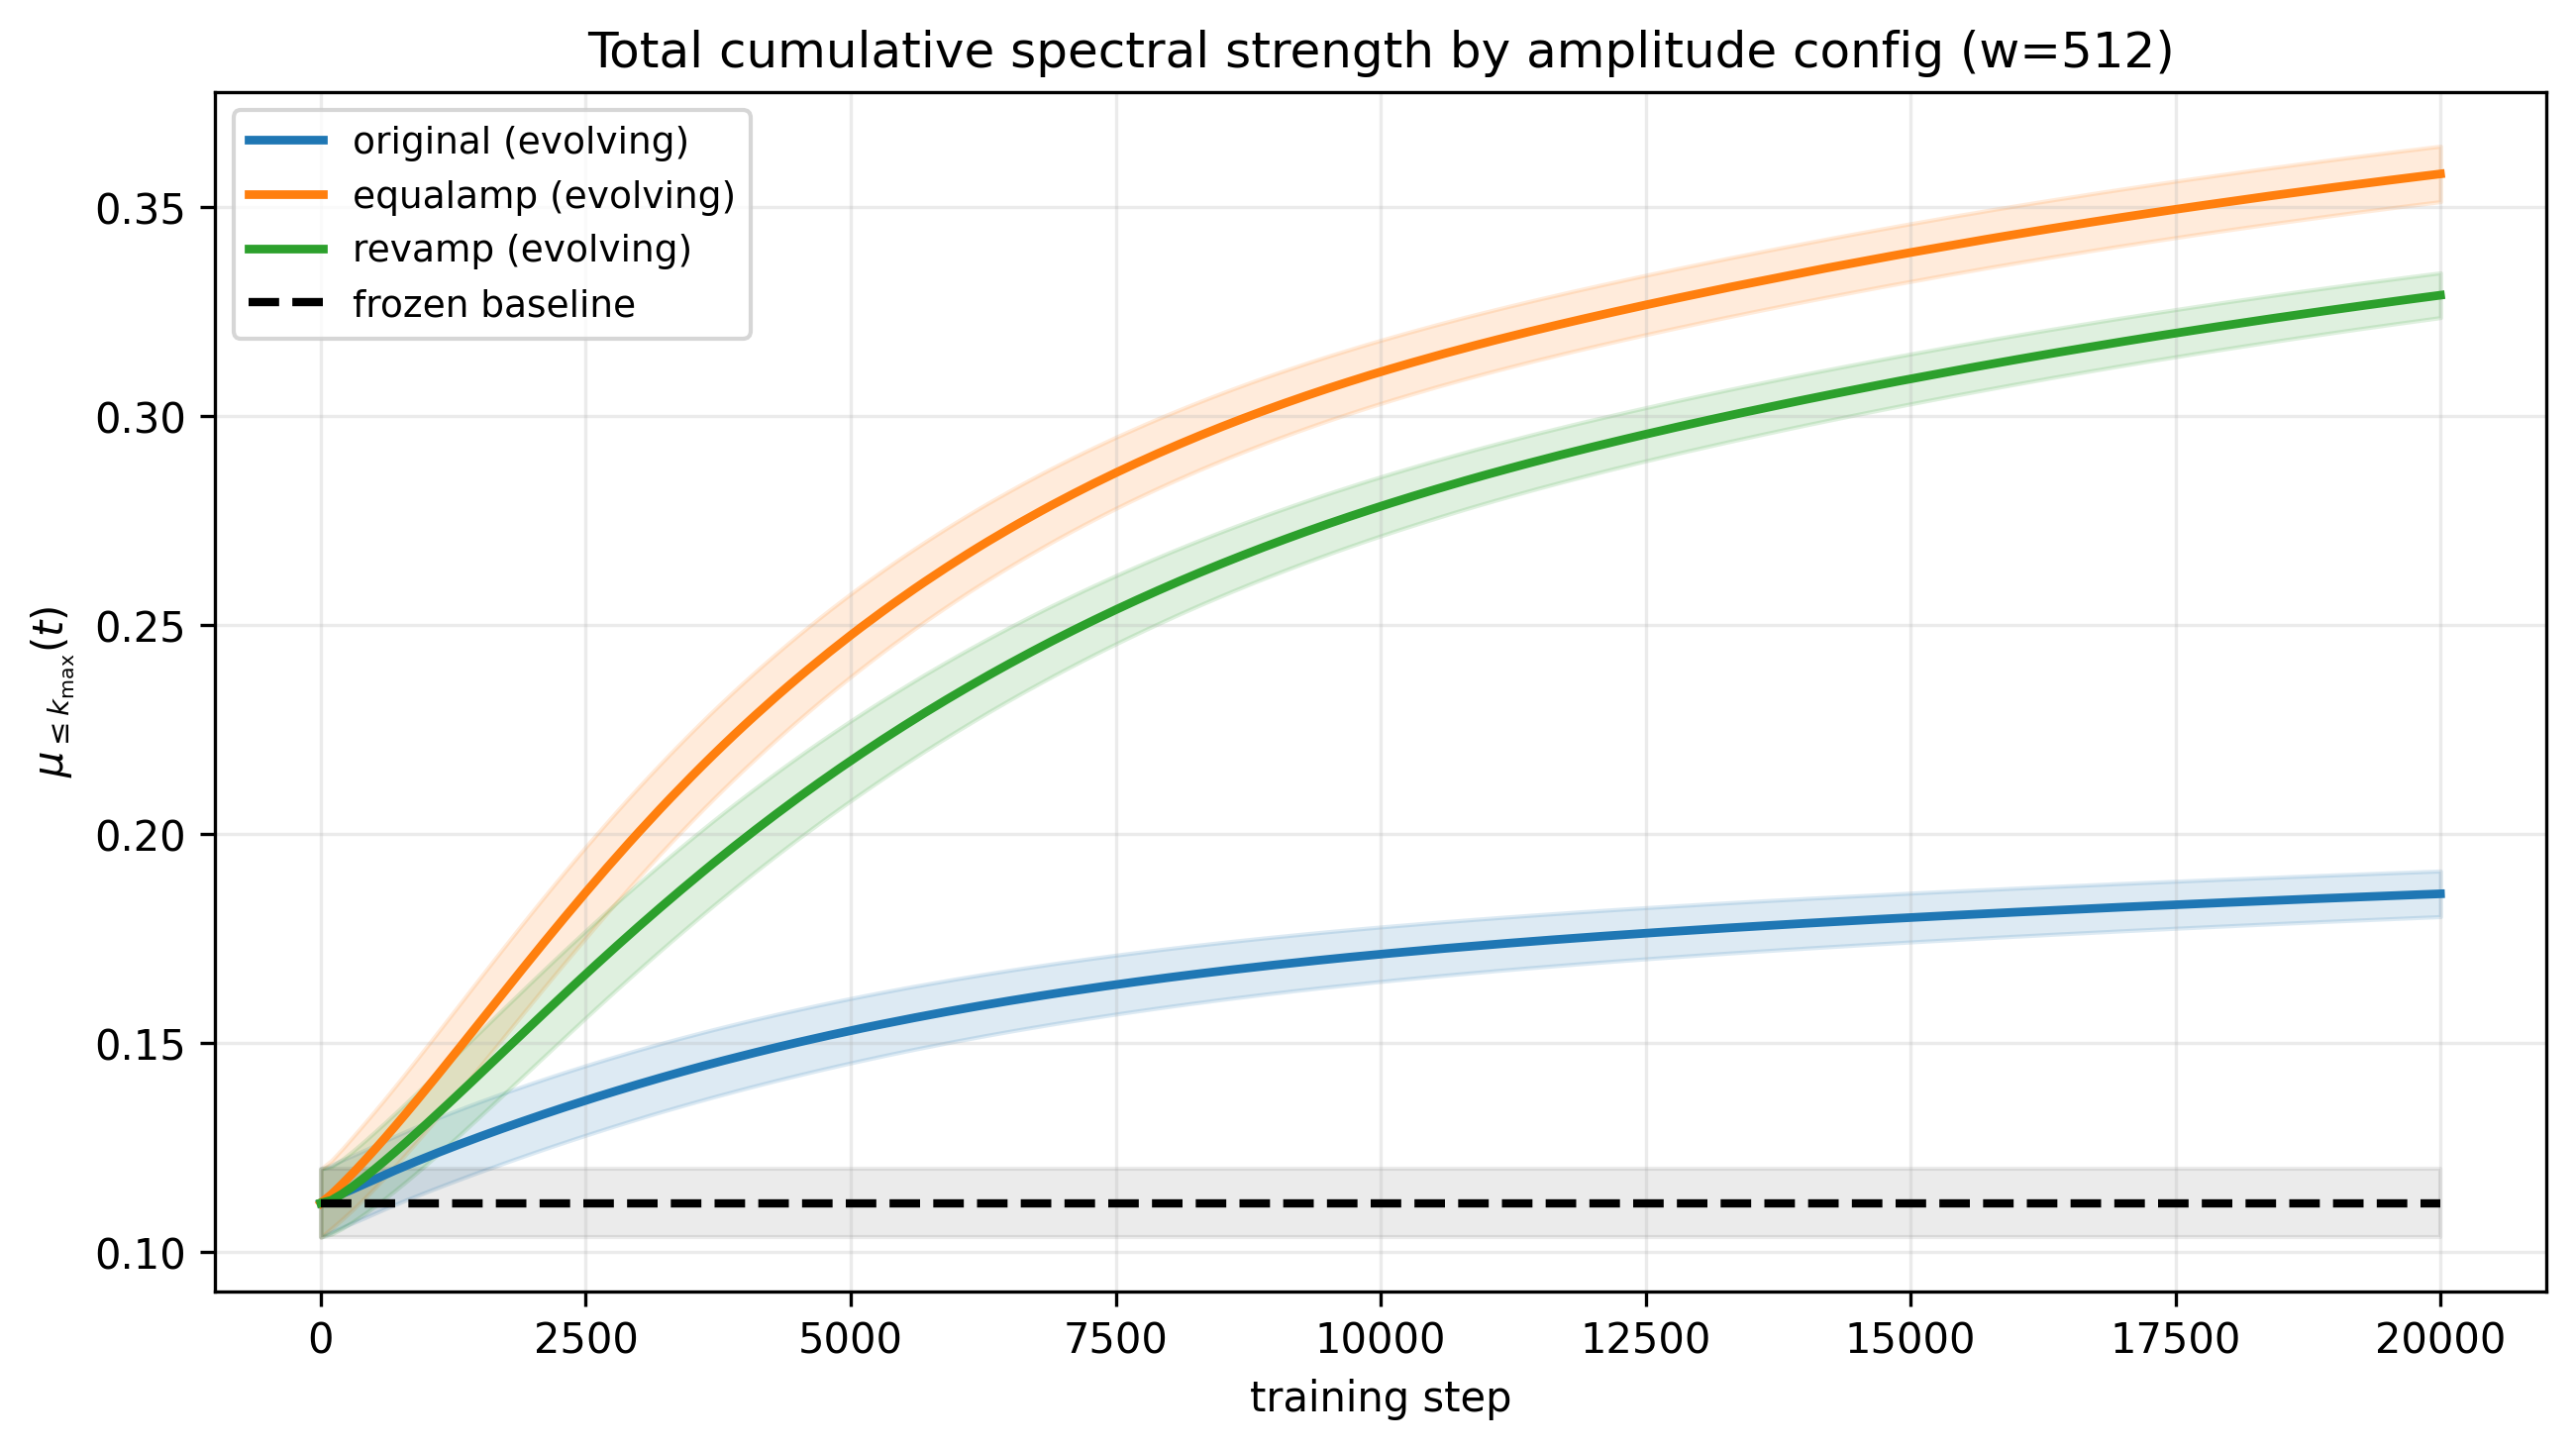
\includegraphics[width=\linewidth]{total_cumulative_mu_amp_configs_w512.png}
		\caption{Width \(512\).}
	\end{subfigure}
	\hfill
	\begin{subfigure}[t]{0.48\textwidth}
		\centering
		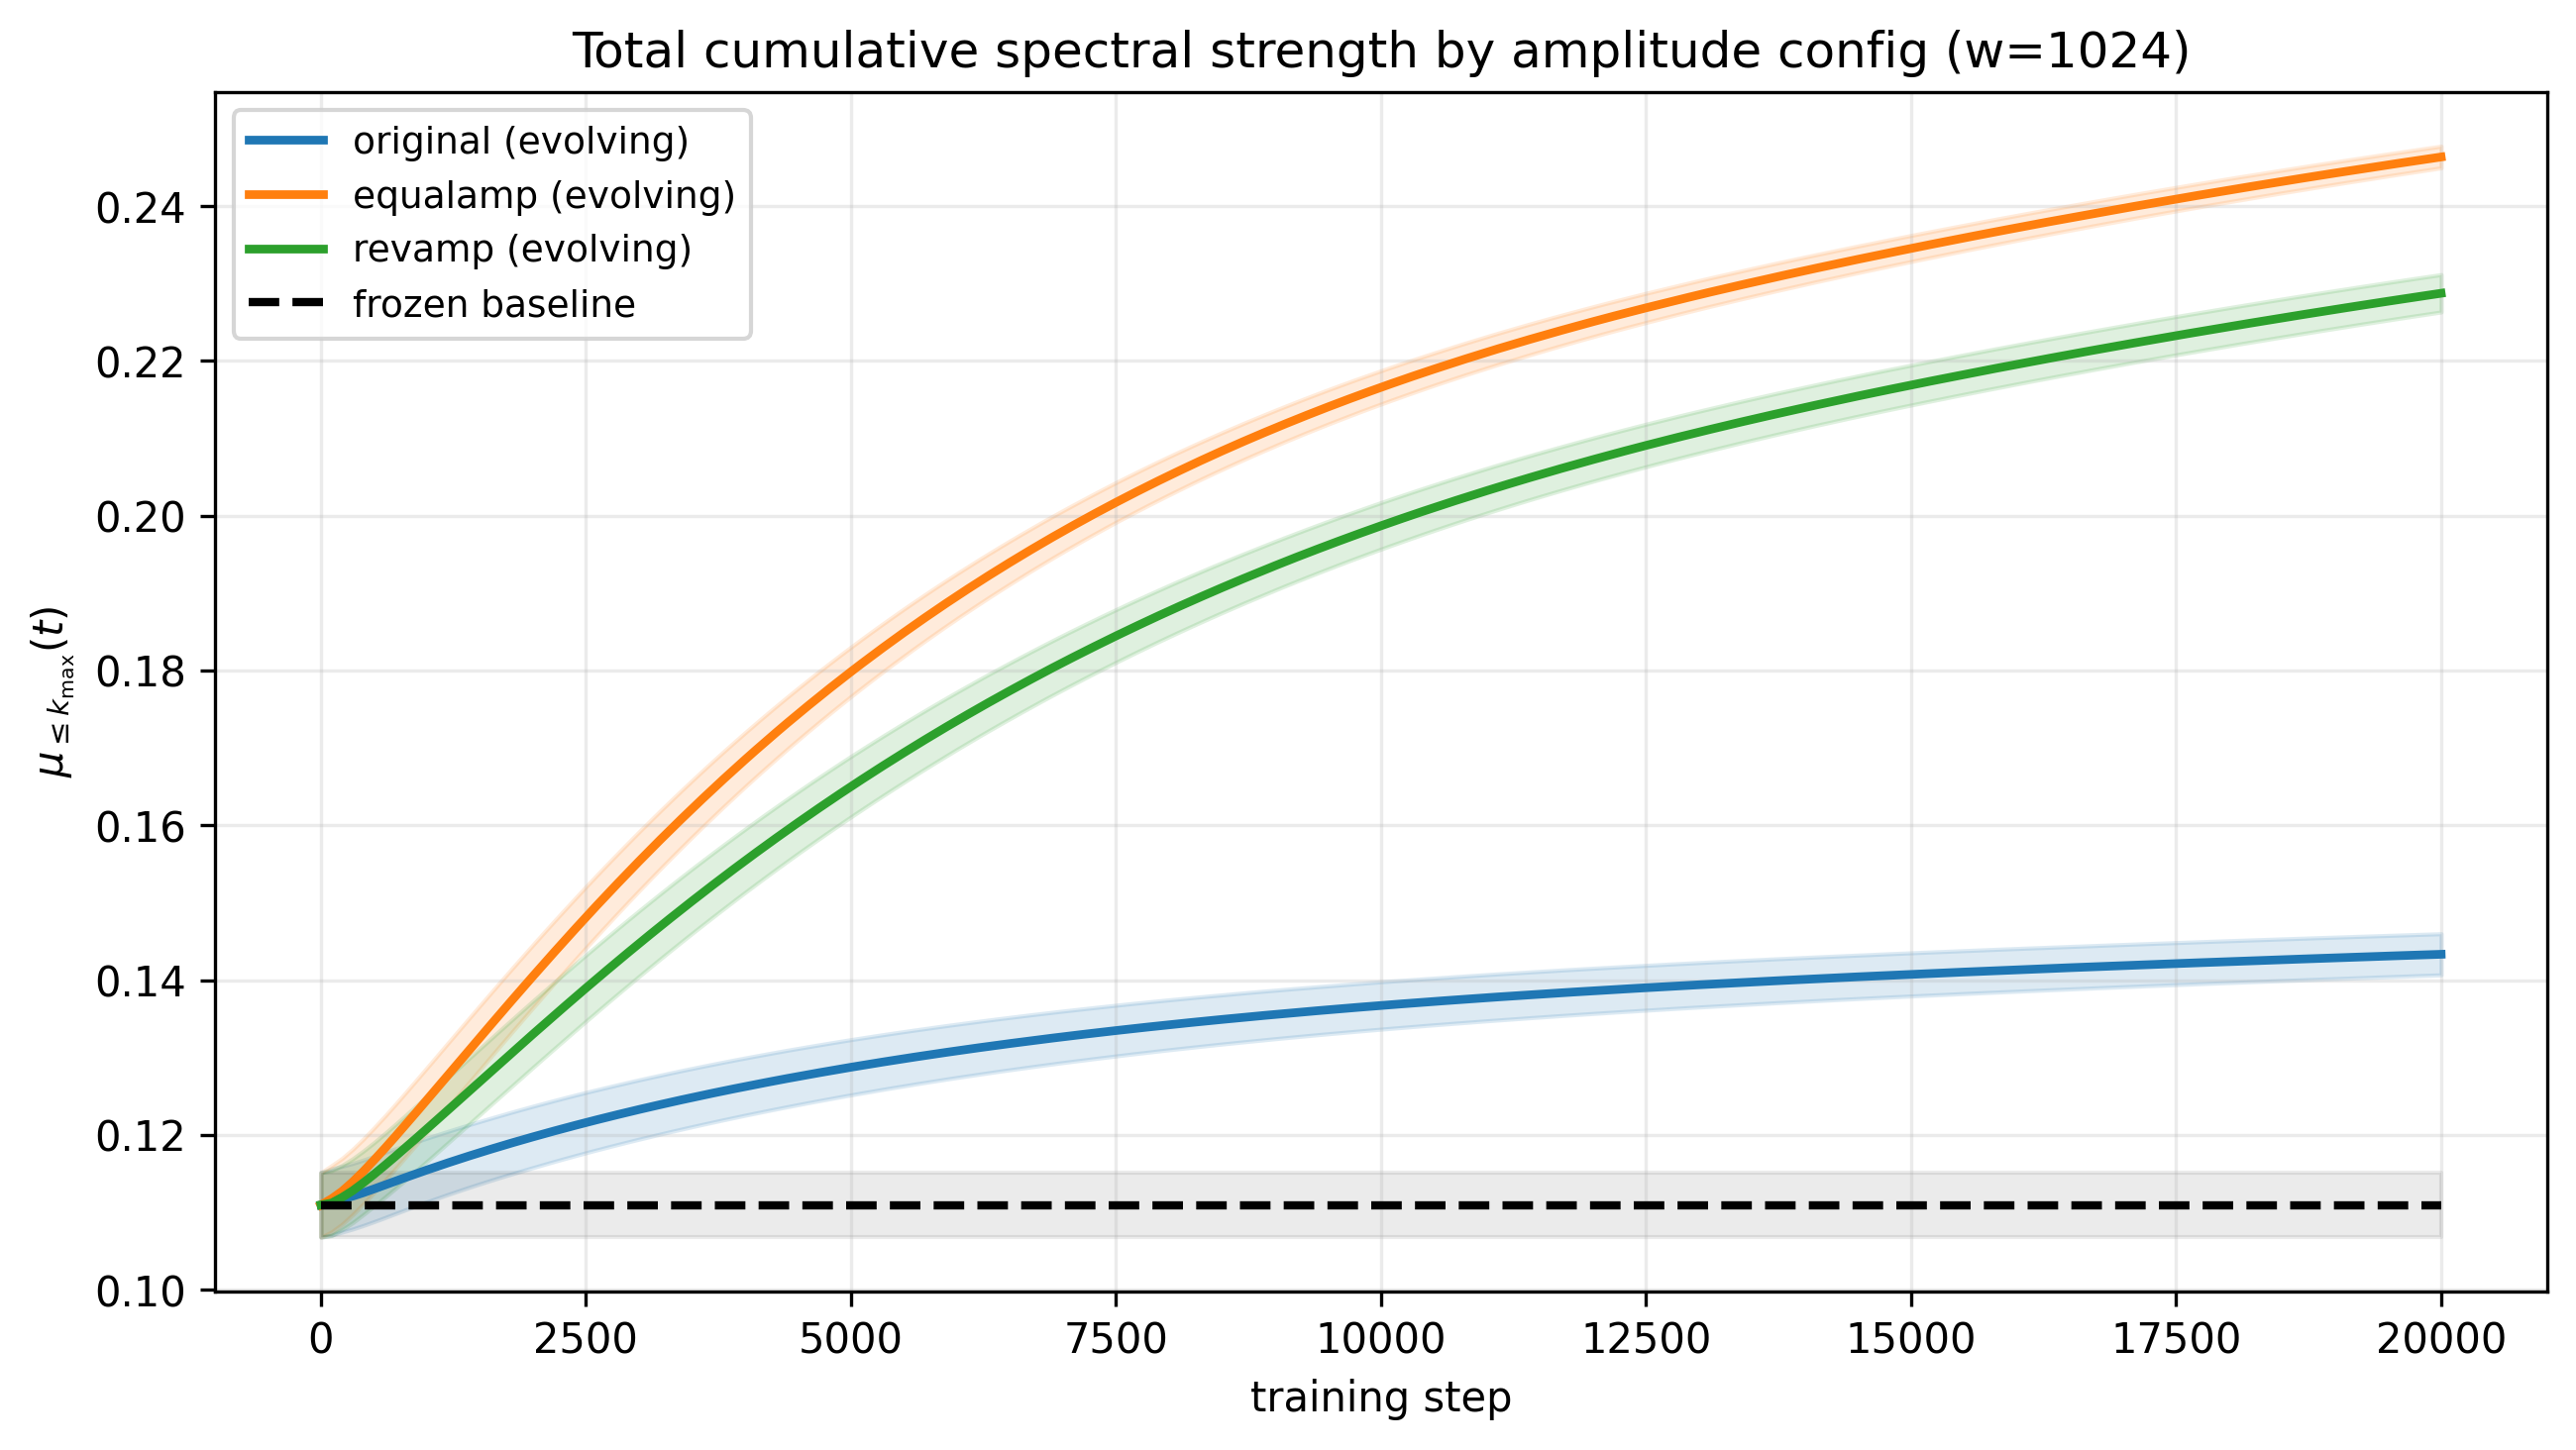
\includegraphics[width=\linewidth]{total_cumulative_mu_amp_configs_w1024.png}
		\caption{Width \(1024\).}
	\end{subfigure}

	\caption{Total cumulative spectral strength across amplitude configurations. The dashed line shows the frozen baseline, while the solid curves show the evolving NTK for the original, equal-amplitude, and reversed-amplitude targets.}
	\label{fig:total-cumulative-spectral-strength}
\end{figure}
\end{document}
